\section*{Appendices}
\renewcommand\thefigure{\thesection\arabic{figure}}    
\counterwithin{figure}{section}
\counterwithin{table}{section}
%\renewcommand{\thesection}{\Alph{section}.\arabic{section}}

\begin{appendices}
%\renewcommand{\appendixtocname}{Annexes} 
\addcontentsline{toc}{section}{Appendices}



% ANNEXE A : SINR determination
\setcounter{figure}{0}
\setcounter{table}{0}
\setcounter{section}{0}
\setcounter{equation}{0}
\numberwithin{equation}{section}
\renewcommand{\theparagraph}{A}

\section{SINR derivation}\label{appA:SINR_deriv}
Let $A$ and $B$ be 2 \gls{rv}'s. These basics properties will be used:
\begin{equation}
    \begin{split}
        &\EX{\alpha A + \beta B} = \alpha \EX{A} + \beta \EX{B} \; \;\; \;\alpha,\beta\in\R \\
        &\EX{AB} = \EX{A} \EX{B} \; \;\; \; \text{if $A$ and $B$ are independent} \\
        &\EX{AB} = \EX{A} \EX{B} + \text{cov}(A,B)\; \; \; \;\text{if $A$ and $B$ are correlated}
    \end{split} 
\end{equation}
\subsection{At the intended position}
As a recall, the received sequence is given by:
\begin{equation}
    \textbf{y}_{\text{B}}^H = \sqrt{\alpha} \; \spread^H \module{\HB}^2 \spread \textbf{x} \;  +  \;  \spread^H \textbf{v}_\text{B} 
    \label{eq:app:rx_bob_AN}
\end{equation}

\paragraph*{Data component}
From (\ref{eq:RV_sinr_b}) and (\ref{eq:expected_bob}), we have:

\begin{subequations}
    \begin{align}
        \EX{|k|^2} &= \EX{\module{\sqrt{\alpha}\spread^H \module{\HB}^2 \spread}^2} \\
        \EX{|k_n|^2} &=\EX{\left|\frac{\sqrt{\alpha}}{U}\sum_{i=0}^{U-1} \left| h_{\text{B}, n + iN}\right|^2\right|^2}  \\
        &= \frac{\alpha}{U^2} \EX{\left(\sum_{i=0}^{U-1} \left| h_{\text{B}, n + iN}\right|^2\right) \left(\sum_{j=0}^{U-1} \left| h_{\text{B}, n + jN}\right|^2\right)^H} \label{subeq:appA:comp1}\\
        &= \frac{\alpha}{U^2}\EX{\sum_{i=0}^{U-1}\sum_{j=0}^{U-1}\left| h_{\text{B}, n + iN}\right|^2 | h^*_{\text{B}, n + jN}|^2} \\
        &= \frac{\alpha}{U^2}\EX{\sum_{i=0}^{U-1}\left| h_{\text{B}, n + iN}\right|^4 + \sum_{i=0}^{U-1}\sum_{\substack{j=0 \\ j\neq i}}^{U-1}\left| h_{\text{B}, n + iN}\right|^2 | h^*_{\text{B}, n + jN}|^2} \\
        &= \frac{\alpha}{U^2} \left(\EX{\sum_{i=0}^{U-1}\left| h_{\text{B}, n + iN}\right|^4} + \EX{\sum_{i=0}^{U-1}\sum_{\substack{j=0 \\ j\neq i}}^{U-1}\left| h_{\text{B}, n + iN}\right|^2 | h^*_{\text{B}, n + jN}|^2} \right) \\
        &=  \frac{\alpha}{U^2} \left(\EX{\sum_{i=0}^{U-1}\left| h_{\text{B}, n + iN}\right|^4} + \EX{\sum_{i=0}^{U-1}\left| h_{\text{B}, n + iN}\right|^2}\EX{\sum_{\substack{j=0 \\ j\neq i}}^{U-1} | h^*_{\text{B}, n + jN}|^2} \right) \label{eq:an_2g}\\
        &= \frac{\alpha}{U^2} \left( 2U + U(U-1)\right) = \frac{\alpha (U+1)}{U} \label{eq:an_2h}
    \end{align}
    \label{eq:appA:data_bob}
\end{subequations}
Going from (\ref{eq:an_2g}) to (\ref{eq:an_2h}) can be deduced from Appendix \ref{appC}. It is then easy to show that $\EX{\left| h_{\text{B}, n + iN}\right|^4}=2$. 

\paragraph*{Additive white gaussian noise component}
We compute the mean energy per symbol of the received noise signal:
\begin{subequations}
    \begin{align}
        \EX{|\textbf{v}_{\text{B}}|^2} &=  \EX{\module{\spread^H \vb}^2} \\
        &= \EX{\left(\spread^H \vb \right)\left(\spread^H \vb \right)^H} \\
        &=\EX{\spread^H \vb \vb^* \spread } \\
        \EX{|v_{\text{B,n}}|^2} &= \frac{1}{U} \EX{\sum_{i=0}^{U-1} |v_{\text{B}, n + iN}|^2} = \sigma^2_{\text{V,B}}
    \end{align}
    \label{eq:appA:noise_bob}
\end{subequations}

       % &\EX{|x_n|^2} = 1\\
       % &\EX{|v_{B,n}|^2} = \sigma^2_{V,E}



\subsection{At the unintended position}
At the unintended position, the received signal is given by:
\begin{equation}
    \textbf{y}_{\text{E}}^G = \sqrt{\alpha} \textbf{G}\Gamma_{\text{E}} \textbf{x} + \sqrt{1-\alpha} \textbf{G} \HE \w + \ve
    \label{eq:appA_rx_eve}
\end{equation}
where $\Gamma_{\text{E}} = \HE \HB^*\spread$




\subsubsection{Eve and Bob with identical capacities}
In this scenario, we have:
\begin{equation}
    \textbf{y}_{\text{E}}^G = \sqrt{\alpha} \spread^H \Gamma_{\text{E}} \spread\; \textbf{x} \; +  \; \sqrt{1-\alpha} \; \spread^H \HE \w  \; +  \; \spread^H  \textbf{v}_\text{E} 
    \label{eq:app:rx_eve_filt0}
\end{equation}


\paragraph*{Data component}
From (\ref{eq:expected_eve_filt0}), we have:
\begin{subequations}
    \begin{align}
        \EX{|\textbf{A}_{1}|^2} &= \EX{\module{\sqrt{\alpha}\spread^H \HE\HB^* \spread}^2} \\
        &= \alpha \EX{\left( \spread^H \HE\HB^* \spread \right) \left( \spread^H \HE\HB^* \spread\right)^H} \\
        \EX{|A_{1,n}|^2}&=\alpha \EX{\frac{1}{U^2} \sum_{i=0}^{U-1} \left| h_{\text{E}, n + iN} \right|^2 \left| h^*_{\text{B}, n + iN}\right|^2 } \\
        &= \frac{\alpha}{U}
    \end{align}
    \label{eq:appA:data_eve_filt0}
\end{subequations}

\paragraph*{Additive white gaussian noise component}
For the noise component:
\begin{subequations}
    \begin{align}
        \EX{|\textbf{A}_{2}|^2} &=  \EX{\module{\spread^H \ve}^2} \\
        &= \EX{\left(\spread^H \ve \right)\left(\spread^H \ve \right)^H} \\
        &=\EX{\spread^H \ve \ve^* \spread } \\
        \EX{|A_{2,n}|^2} &= \frac{1}{U} \EX{\sum_{i=0}^{U-1} |v_{\text{E}, n + iN}|^2} = \sigma^2_{\text{V,E}}
    \end{align}
    \label{eq:appA:noise_eve_filt0}
\end{subequations}

\paragraph*{Artificial noise component}
The \gls{an} term is given by:
\begin{subequations}
    \begin{align}
        \EX{|\textbf{A}_{3}|^2} &=  \EX{\module{\sqrt{1-\alpha}\spread^H \HE \w}^2} \\
        &= (1-\alpha)\EX{\left(\spread^H \HE \w \right)\left(\spread^H \HE\w \right)^H} \\
        &=(1-\alpha)\EX{\spread^H \HE\textbf{H}^*_{\text{E}} \w\w^* \spread } \\
        \EX{|A_{3,n}|^2}  &= \frac{1-\alpha}{U} \EX{\sum_{i=0}^{U-1} |h_{\text{E}, n + iN}w_{n + iN}|^2} = (1-\alpha)\sigma^2_{\text{AN}}
    \end{align}
    \label{eq:appA:an_eve_filt0}
\end{subequations}



\subsubsection{Matched Filtering}
When Eve performs a matched filtering with the received signal, we obtain:
\begin{equation}
    \textbf{y}_{\text{E}}^G = \sqrt{\alpha} \spread^H \module{\HE}^2 \module{\HB}^2 \spread\; \textbf{x} \; +  \; \sqrt{1-\alpha} \; \spread^H \HB\module{\HE}^2 \w  \; +  \; \spread^H  \textbf{H}^*_E \textbf{H}_B \;\ve
    \label{eq:appA:rx_eve_filt1}
\end{equation}

\paragraph*{Data component}
The data component is given by:
\begin{subequations}
    \begin{align}
        \EX{|\textbf{A}_{1}|^2} &= \EX{\module{\sqrt{\alpha} \spread^H \module{\HE}^2 \module{\HB}^2 \spread\; \textbf{x}}^2} \\
        &= \alpha \EX{\module{ \spread^H \module{\HE}^2 \module{\HB}^2 \spread}^2} \EX{|\textbf{x}|^2} \\
        \EX{|A_{1,n}|^2} &= \alpha \EX{\left|\frac{1}{U}\sum_{i=0}^{U-1} \left| h_{\text{B}, n + iN}\right|^2 \left| h_{\text{E}, n + iN}\right|^2\right|^2} \\
        &=  \frac{\alpha}{U^2} \EX{\left(\sum_{i=0}^{U-1} \left| h_{\text{B}, n + iN}\right|^2 \left| h_{\text{E}, n + iN}\right|^2 \right) \left(\sum_{j=0}^{U-1} \left| h_{\text{B}, n + jN}\right|^2 \left| h_{\text{E}, n + iN}\right|^2 \right)^H} \label{subeq:appA_comp2} \\
        &= \frac{\alpha}{U^2} \EX{\sum_{i=0}^{U-1}\sum_{j=0}^{U-1} \left| h_{\text{B}, n + jN}\right|^2 \left| h_{\text{E}, n + iN}\right|^2 \left| h^*_{\text{B}, n + jN}\right|^2 \left| h^*_{\text{E}, n + iN}\right|^2} \\
        &= \frac{\alpha}{U^2}\left( \sum_{i=0}^{U-1} \left| h_{\text{B}, n + jN}\right|^4 \left| h_{\text{E}, n + iN}\right|^4 + \sum_{i=0}^{U-1}\sum_{\substack{j=0 \\ j\neq i}}^{U-1}  \left| h_{\text{B}, n + jN}\right|^2 \left| h_{\text{E}, n + iN}\right|^2 \left| h^*_{\text{B}, n + jN}\right|^2 \left| h^*_{\text{E}, n + iN}\right|^2 \right) \\
        &= \frac{\alpha}{U^2} \left(U.2.2 + U(U-1) \right) = \frac{\alpha (U+3)}{U}
        \label{subeq:appA_match_final}
     \end{align} 
    \label{eq:appA:data_eve_filt1}
\end{subequations}
We remark that (\ref{subeq:appA_comp2}) can be directly computed from (\ref{subeq:appA:comp1}), which leads to (\ref{subeq:appA_match_final}).\\



\paragraph*{Additive white gaussian noise component}
The noise component is:
\begin{subequations}
    \begin{align}
        \EX{|\textbf{A}_{2}|^2} &=  \EX{\module{\spread^H \HE^* \HB \ve}^2} \\
        &= \EX{\left(\spread^H \HE^* \HB \ve \right)\left(\spread^H \HE^* \HB \ve \right)^H} \\
        &=\EX{\spread^H   \HE \HE^* \HB\HB^*  \ve \ve^* \spread } \\
       \EX{|A_{2,n}|^2} &= \frac{1}{U} \EX{\sum_{i=0}^{U-1} |h_{\text{E}, n + iN}|^2 |h_{\text{B}, n + iN}|^2 |v_{\text{E}, n + iN}|^2} = \sigma^2_{\text{V,E}}
    \end{align}
    \label{eq:appA:noise_eve_filt1}
\end{subequations}




\paragraph*{Artificial noise component}
We want to compute the mean energy per symbol received at Eve for the \gls{an} component when she performs a matched filtering. The \gls{an} term at Eve is given by:
\begin{subequations}
\begin{align}
\vect{v}&=	\mat{S}^H \mat{H}_B |\mat{H}_E|^2 \vect{w} \label{eq:an_decod1_a}\\
&=\mat{A} |\mat{H}_E|^2 \mat{V}_2 \vect{w}' \label{eq:an_decod1_b}\\
&= \mat{U} \begin{pmatrix}
\mat{\Sigma} & \mat{0}_{Q-N\times N}
\end{pmatrix}  \begin{pmatrix}
\mat{V}_1^H\\
\mat{V}_2^H
\end{pmatrix} |\mat{H}_E|^2 \mat{V}_2 \vect{w}'\\
&=\mat{U} \mat{\Sigma}\mat{V}_1^H |\mat{H}_E|^2 \mat{V}_2 \vect{w}'
\end{align}
\end{subequations}
where:
\begin{itemize}
	\item $\mat{U}$ is a $N \times N$ unitary matrix, i.e., $\mat{U}^H \mat{U} = \mat{I}_N$, its columns form an orthonormal basis of $\mathcal{C}^N$ and are the left singular vectors of each singular value of $\mat{A}$;
	\item $\mat{\Sigma}$ is a $N \times N$ diagonal matrice containing the singular values of $\mat{A}$ in the descending order, i.e., $\sigma_i = \mat{\Sigma}_{i,i}$;
	\item $\mat{V}_1$ is a $Q \times N$ complex matrix that contains the right singular vectors associated to the non-zero singular values;
	\item $\mat{V}_2$ is a $Q \times Q-N$ complex matrix that contains the right singular vectors associated to the zeroes singular values, i.e., that span the right null-space of $\mat{A}$;
	\item $\mat{V} = \left(\mat{V}_1 \; \mat{V}_2\right)$ is a $Q \times Q$ unitary matrix, i.e., $\mat{V}^H \mat{V} = \mat{I}_Q$, its columns form an orthonormal basis of $\mathcal{C}^Q$ and are the right singular vectors of each singular value of $\mat{A}$;
	\item $\vect{w'}$ is a $Q-N \times 1$ complex normal random variable such that $\vect{w'} \sim \mathcal{CN}(0,1)$
\end{itemize} 
Note that going from (\ref{eq:an_decod1_a}) to (\ref{eq:an_decod1_b}), we deliberately omit the weighting coefficient $\beta$ appearing in (\ref{eq:an_w}) for the sake of simplicity. The value of this coefficient will be given at the end of the discussion.


Let us now look at the covariance matrix
\begin{subequations}
\begin{align}
\mathbb{E}\left(\vect{v}\vect{v}^H\right)&=\mathbb{E}\left(\mat{U} \mat{\Sigma}\mat{V}_1^H |\mat{H}_E|^2 \mat{V}_2 \vect{w}'\left(\mat{U} \mat{\Sigma}\mat{V}_1^H |\mat{H}_E|^2 \mat{V}_2 \vect{w}'\right)^H\right)\\
&=\mathbb{E}\left(\mat{U} \mat{\Sigma}\mat{V}_1^H |\mat{H}_E|^2 \mat{V}_2 \vect{w}'\vect{w}'^H\mat{V}_2^H|\mat{H}_E|^2\mat{V}_1 \mat{\Sigma}^H   \mat{U}^H\right)
\end{align}
\end{subequations}

Note that $\vect{w}'$ is independent of other random variables and has a unit covariance matrix. We can thus put the expectation inside to get
\begin{align}
\mathbb{E}\left(\vect{v}\vect{v}^H\right)&=\mathbb{E}\left(\mat{U} \mat{\Sigma}\mat{V}_1^H |\mat{H}_E|^2 \mat{V}_2 \mat{V}_2^H|\mat{H}_E|^2\mat{V}_1 \mat{\Sigma}^H   \mat{U}^H\right)
\end{align}


We rewrite $|\mat{H}_E|^2=\sum_{q=1}^Q|H_{E,q}|^2 \vect{e}_q \vect{e}_q^T $ where $\vect{e}_q$ is an all zero vector except a $1$ at row $q$ to isolate the independent random variable $H_E$

\begin{subequations}
\begin{align}
\mathbb{E}\left(\vect{v}\vect{v}^H\right)&=\sum_{q=1}^Q\sum_{q'=1}^Q\mathbb{E}(|H_{E,q}|^2|H_{E,q'}|^2)\mathbb{E}\left(\mat{U} \mat{\Sigma}\mat{V}_1^H  \vect{e}_q \vect{e}_q^T \mat{V}_2 \mat{V}_2^H \vect{e}_{q'} \vect{e}_{q'}^T\mat{V}_1 \mat{\Sigma}^H   \mat{U}^H\right)\\
&=\sum_{q=1}^Q\mathbb{E}(|H_{E,q}|^4)\mathbb{E}\left(\mat{U} \mat{\Sigma}\mat{V}_1^H  \vect{e}_q \vect{e}_q^T \mat{V}_2 \mat{V}_2^H \vect{e}_{q} \vect{e}_{q}^T\mat{V}_1 \mat{\Sigma}^H   \mat{U}^H\right)\\
&+\sum_{q=1}^Q\sum_{q'\neq q}^Q\mathbb{E}(|H_{E,q}|^2|H_{E,q'}|^2)\mathbb{E}\left(\mat{U} \mat{\Sigma}\mat{V}_1^H  \vect{e}_q \vect{e}_q^T \mat{V}_2 \mat{V}_2^H \vect{e}_{q'} \vect{e}_{q'}^T\mat{V}_1 \mat{\Sigma}^H   \mat{U}^H\right)\\
&=2\sum_{q=1}^Q\mathbb{E}\left(\mat{U} \mat{\Sigma}\mat{V}_1^H  \vect{e}_q \vect{e}_q^T \mat{V}_2 \mat{V}_2^H \vect{e}_{q} \vect{e}_{q}^T\mat{V}_1 \mat{\Sigma}^H   \mat{U}^H\right)\\
&+\sum_{q=1}^Q\sum_{q'\neq q}^Q\mathbb{E}\left(\mat{U} \mat{\Sigma}\mat{V}_1^H  \vect{e}_q \vect{e}_q^T \mat{V}_2 \mat{V}_2^H \vect{e}_{q'} \vect{e}_{q'}^T\mat{V}_1 \mat{\Sigma}^H   \mat{U}^H\right)\\
&=\sum_{q=1}^Q\mathbb{E}\left(\mat{U} \mat{\Sigma}\mat{V}_1^H  \vect{e}_q \vect{e}_q^T \mat{V}_2 \mat{V}_2^H \vect{e}_{q} \vect{e}_{q}^T\mat{V}_1 \mat{\Sigma}^H   \mat{U}^H\right)\\
&+\mathbb{E}\left(\mat{U} \mat{\Sigma}\mat{V}_1^H \sum_{q=1}^Q \vect{e}_q \vect{e}_q^T \mat{V}_2 \mat{V}_2^H \sum_{q'=1}^Q\vect{e}_{q'} \vect{e}_{q'}^T\mat{V}_1 \mat{\Sigma}^H   \mat{U}^H\right)\\
&=\sum_{q=1}^Q\mathbb{E}\left(\mat{U} \mat{\Sigma}\mat{V}_1^H  \vect{e}_q \vect{e}_q^T \mat{V}_2 \mat{V}_2^H \vect{e}_{q} \vect{e}_{q}^T\mat{V}_1 \mat{\Sigma}^H   \mat{U}^H\right)+\mathbb{E}\left(\mat{U} \mat{\Sigma}\mat{V}_1^H  \mat{V}_2 \mat{V}_2^H \mat{V}_1 \mat{\Sigma}^H   \mat{U}^H\right)
\end{align}
\end{subequations}

Using the fact that $\mat{V}_2^H \mat{V}_1=\mat{0}$, the second term cancels and
\begin{align}
\mathbb{E}\left(\vect{v}\vect{v}^H\right)&=\mathbb{E}\left(\mat{U} \mat{\Sigma}\mat{V}_1^H  \sum_{q=1}^Q\left(\vect{e}_q \vect{e}_q^T \mat{V}_2 \mat{V}_2^H \vect{e}_{q} \vect{e}_{q}^T\right)\mat{V}_1 \mat{\Sigma}^H   \mat{U}^H\right)
\end{align}

Since all elements of $\vect{v}$ have same variance, we can compute it as
\begin{subequations}
\begin{align}
\frac{1}{N}\mathbb{E}\left(\|\vect{v}\|^2\right)&=\frac{1}{N}\mathbb{E}\ \tr\left(\vect{v}\vect{v}^H\right)\\
&=\frac{1}{N}\mathbb{E} \ \tr\left( \mat{\Sigma}^2\mat{V}_1^H  \sum_{q=1}^Q\left(\vect{e}_q \vect{e}_q^T \mat{V}_2 \mat{V}_2^H \vect{e}_{q} \vect{e}_{q}^T\right)\mat{V}_1 \right)
\end{align}
\end{subequations}

Let us rewrite $\mat{V}_1=\sum_{l}\vect{e}_{l}\vect{v}_{1,l}^H$ where $\vect{v}_{1,l}^H$ is the $l$-th row of $\mat{V}_1$ (of dimension $N\times 1$) with only one nonzero element.
\begin{subequations}
\begin{align}
\frac{1}{N}\mathbb{E}\left(\|\vect{v}\|^2\right)&=\frac{1}{N}\sum_{q=1}^Q\sum_{l}\sum_{l'}\mathbb{E} \ \tr\left( \mat{\Sigma}^2\vect{v}_{1,l}\vect{e}_{l'}^T  \vect{e}_q \vect{e}_q^T \mat{V}_2 \mat{V}_2^H \vect{e}_{q} \vect{e}_{q}^T\vect{e}_{l}\vect{v}_{1,l}^H \right)\\
&=\frac{1}{N}\sum_{q=1}^Q\sum_{l}\sum_{l'}\delta_{l'-q}\delta_{l-q} \mathbb{E} \ \tr\left( \mat{\Sigma}^2\vect{v}_{1,l}\vect{e}_q^T \mat{V}_2 \mat{V}_2^H \vect{e}_{q} \vect{v}_{1,l}^H \right)\\
&=\frac{1}{N}\sum_{q=1}^Q \mathbb{E} \ \tr\left( \mat{\Sigma}^2\vect{v}_{1,q}\vect{e}_q^T \mat{V}_2 \mat{V}_2^H \vect{e}_{q} \vect{v}_{1,q}^H \right)
\end{align}
\end{subequations}

Let us rewrite $\mat{V}_2=\sum_{l}\vect{e}_{l}\vect{v}_{2,l}^H$ where $\vect{v}_{2,l}^H$ is the $l$-th row of $\mat{V}_2$ (of dimension $Q-N\times 1$) with $U-1$ nonzero elements

\begin{subequations}
\begin{align}
\frac{1}{N}\mathbb{E}\left(\|\vect{v}\|^2\right)&=\frac{1}{N}\sum_{q=1}^Q\sum_l\sum_{l'} \mathbb{E} \ \tr\left( \mat{\Sigma}^2\vect{v}_{1,q}\vect{e}_q^T \vect{e}_{l}\vect{v}_{2,l}^H \vect{v}_{2,l'} \vect{e}_{l'}^T \vect{e}_{q} \vect{v}_{1,q}^H \right)\\
&=\frac{1}{N}\sum_{q=1}^Q \mathbb{E} \ \tr\left( \mat{\Sigma}^2\vect{v}_{1,q}\vect{v}_{2,q}^H \vect{v}_{2,q} \vect{v}_{1,q}^H \right)\\
&=\frac{1}{N}\sum_{q=1}^Q \mathbb{E} \left( \| \vect{v}_{2,q}\|^2\vect{v}_{1,q}^H\mat{\Sigma}^2\vect{v}_{1,q}  \right)
\end{align}
\end{subequations}

where $\vect{v}_{1,q}^H \mat{\Sigma}^2 \vect{v}_{1,q} \coloneqq  \| \vect{v}_{1,q}\|^2 \sigma_n^2$ is a scalar. Therefore, we obtain:

\begin{align}
\frac{1}{N}\mathbb{E}\left(\|\vect{v}\|^2\right) &=\frac{1}{N}\sum_{q=1}^Q \mathbb{E} \left( \| \vect{v}_{2,q}\|^2 \| \vect{v}_{1,q}\|^2 \sigma_n^2  \right)
\end{align}


Since $\mat{V}$ forms an orthonormal basis, i.e., $\mat{V}^H \mat{V} = \mat{I}_Q$, we have $ \| \vect{v}_{1,q}\|^2 +  \| \vect{v}_{2,q}\|^2 = 1$. We then have:
\begin{align}
\frac{1}{N}\mathbb{E}\left(\|\vect{v}\|^2\right) &=\frac{1}{N}\sum_{q=1}^Q \mathbb{E} \left[ \left( \| \vect{v}_{1,q}\|^2 - \| \vect{v}_{1,q}\|^4 \right) \sigma_n^2  \right]
\label{eq:v_1}
\end{align}

To determine (\ref{eq:v_1}), we need to know the transformations performed by the singular value decomposition on the input matrix $\mat{A}$ to obtain $\vect{v}_{1,q}$ and $\sigma^2_n$, i.e., we have to find an analytic expression of $\vect{v}_{1,q}$ and $\sigma^2_n$. We know that:

\begin{equation}
\resizebox{\textwidth}{!}{
\mat{A} = \mat{S}^H\mat{H}_B = 
\begin{bmatrix}
z_1 & 0 & \hdots & 0 & z_2 & 0 & \hdots & 0 & \hdots & z_U & 0 & \hdots & 0\\
0 & z_{U+1} & \hdots & 0 & 0 & z_{U+2} & \hdots & 0 & \hdots &0 & z_{2U} & \hdots & 0 \\
\vdots & & \ddots & \vdots &\vdots & &\ddots & \vdots & \hdots & \vdots &  & \ddots & \vdots \\
0 & 0 & \hdots & z_{(N-1)U+1} & 0 & 0 & \hdots & z_{(N-1)U+2}&  \hdots &0 &0 &\hdots & z_Q
\end{bmatrix}}
\end{equation}
where $\mat{A} \in \mathcal{C}^{N\times Q}$ and $z_i  = z_{i,x} + jz_{i,y} \sim \mathcal{CN}(0,\frac{1}{U}) \sim \mathcal{N}(0,\frac{1}{2U}) + j \mathcal{N}(0,\frac{1}{2U})$. After singular value decomposition, we obtain:

\begin{equation}
\mat{\Sigma} =
\begin{bmatrix}
\sigma_1 & 0 &\hdots & 0 \\
0 & \sigma_2 & \hdots & 0 \\
\vdots &  &\ddots &  \vdots \\
0 & 0 & \hdots & \sigma_N
\end{bmatrix}
\end{equation}
where $\sigma_n = \sqrt{\sum_{i=1}^{U} \left| z_{(n-1)U+i}\right|^2} \; , n = 1...N$
\begin{equation}
\mat{V}_1 = 
\begin{bmatrix}
v_1  & 0 & \hdots & 0 \\
0 & v_{U+1} &  \hdots & 0 \\
\vdots & & \ddots &  \vdots \\
0 & 0 & \hdots & v_{(U-1)N+1} \\
v_2 & 0 & \hdots & 0 \\
0  & v_{U+2} & \hdots & 0\\
\vdots & &\ddots &  \vdots\\
0 & 0 & \hdots & v_{(U-1)N+2} \\
\vdots & \vdots & &  \vdots\\	
v_U  & 0 & \hdots & 0 \\
0 & v_{2U} & \hdots & 0 \\
\vdots &  & \ddots & \vdots\\
0 & 0  & \hdots & v_Q
\end{bmatrix}
\end{equation}
where $v_i  = \frac{z_i^*}{\sigma_k}, \; i = 1..Q \; , \; k = 1...N$ represents the column of $\mat{V}_1$ where $v_i$ belongs. \\
From that, we obtain:
\begin{subequations}
\begin{align}
\mathbb{E} \left[\sigma_n^2 \right] &= \mathbb{E}\left[ \sum_{i=1}^{U} \left| z_{(n-1)U+i}\right|^2 \right]  \\
& = U \mathbb{E} \left[ \left| z_{(n-1)U+i}\right|^2 \right] \\
&= U \frac{1}{U} \\
& = 1
\end{align}
\end{subequations}

Without loss of generality, we  compute $\mathbb{E} \left[ \| v_1\|^2 \right]$ and $\mathbb{E} \left[ \| v_1\|^4 \right]$ since all components of $\mat{V}_1$ are identically distributed:

\begin{subequations}
\begin{align}
\mathbb{E} \left[ \| v_1\|^2 \right] &= \mathbb{E}\left[ \left| \frac{z_1^*}{\sigma_1}\right|^2\right]  \\
& =  \mathbb{E} \left[ \frac{\left| z_1 \right|^2 }{\sigma_1^2} \right] \\
&=  \mathbb{E} \left[   \frac{\left| z_1 \right|^2 }{  \sum_{i=1}^{U} \left| z_i\right|^2 }  \right] \\
& = \mathbb{E} \left[   \frac{\left| z_1 \right|^2 }{  U \left| z_1 \right|^2 }  \right] \\
& = \frac{1}{U}
\end{align}
\end{subequations}

For the moment of order 4, we note that $\mathbb{E}\left[ \left| z_i \right|^4\right] = \frac{2}{U^2}$ \footnote{see Appendix \ref{appC}}.
\begin{subequations}
\begin{align}
\mathbb{E} \left[ \| v_1\|^4 \right] &= \mathbb{E}\left[ \left| \frac{z_1^*}{\sigma_1}\right|^4\right] \\
& =  \mathbb{E} \left[ \frac{\left| z_1 \right|^4 }{\sigma_1^4} \right] \\
&=  \mathbb{E} \left[   \frac{\left| z_1 \right|^4 }{  \left( \sum_{i=1}^{U} \left| z_i\right|^2 \right)^2 }  \right] \label{eq:moment_4_1} \\
&= \mathbb{E} \left[   \frac{\left| z_1 \right|^4 }{  \sum_{i=1}^{U} \left| z_i\right|^4 + 2 \sum_{i=1}^{U} \sum_{j<i} \left|z_i\right|^2 \left|z_j\right|^2 }  \right] \label{eq:moment_4_2}\\
&= \mathbb{E} \left[   \frac{\left| z_1 \right|^4 }{ U \left| z_1\right|^4 + 2 \frac{(U-1)U}{2} \left|z_i\right|^2 \left|z_j\right|^2 }  \right] \\
& = \frac{\frac{2}{U^2}}{U\frac{2}{U^2} + 2 \frac{(U-1)U}{2} \frac{1}{U} \frac{1}{U}} \\
& =  \frac{\frac{2}{U^2}}{\frac{U+1}{U}} \\
&= \frac{2}{U(U+1)}
\end{align}
\end{subequations}
The double sum on the denominator of (\ref{eq:moment_4_2}) contains $\frac{(U-1)U}{2}$ double products.\\

Finally, we can compute (\ref{eq:v_1}) as:

\begin{subequations}
\begin{align}
\frac{1}{N}\mathbb{E}\left(\|\vect{v}\|^2\right)&=\frac{1}{N} \sum_{q=1}^{Q} \left[ \left( \frac{1}{U} - \frac{2}{U(U+1)} \right) 1\right] \\
&= \frac{1}{N} Q \frac{U-1}{U(U+1)} \\
&= \frac{U-1}{U+1} \label{eq:final_an_result_no_correction}
\end{align}
\end{subequations}

which is the mean energy per \gls{an} received symbol when Eve implements a matched filter. \\

As previously mentionned, we omitted the weighting coefficient  $\beta$. Without this coefficient, we have $\mathbb{E} \left[ |\vect{w}|^2\right]  = \mathbb{E} \left[ |\mat{V}_2\vect{w}'|^2\right] = \frac{U-1}{U}$.  In the simulation, we assumed $\mathbb{E} \left[ |\vect{w}|^2\right]  = \frac{1}{U}$, such that the coefficient must correct  (\ref{eq:final_an_result_no_correction}) by $\beta = \frac{1}{U-1}$. \\
With the correction taken into account, the final expression for the mean energy per \gls{an} received symbol when Eve implements a matched filter is given by:
\begin{equation}
\frac{1}{N}\mathbb{E}\left(\|\vect{v}\|^2\right)=\frac{1}{U+1} 
\end{equation}










\subsubsection{AN suppression}
In this scenario, the received signal at Eve is given by:
\begin{equation}
    \textbf{y}_{\text{E}}^G = \sqrt{\alpha} \spread^H \module{\HB}^2 \spread\; \textbf{x} \; +  \; \spread^H  \HE^{-1} \textbf{H}_B \;\ve
    \label{eq:appA:rx_eve_filt2}
\end{equation}

\paragraph*{Data component}
In what concerns the data component, the computation is straightforward since it is similar to (\ref{eq:appA:data_bob}). 
We then obtain $ \EX{|A_{1,n}|^2} = \alpha \frac{U+1}{U}$.\\

\paragraph*{Additive white gaussian noise component}
The noise term is:
\begin{subequations}
    \begin{align}
        \EX{|\textbf{A}_{2}|^2} &=  \EX{\module{\spread^H \HB \HE^{-1} \ve}^2} \\
        &= \EX{\left(\spread^H \HB \HE^{-1} \ve \right)\left(\spread^H \HB \HE^{-1} \ve \right)^H} \\
        &=\EX{\spread^H   \module{\HB}^2 \module{\HE^{-1}}^2 \module{\ve}^2 \spread } \\
        \EX{|A_{2,n}|^2} &= \frac{1}{U} \EX{\sum_{i=0}^{U-1} |h_{\text{E}, n + iN}^{-1}|^2 |h_{\text{B}, n + iN}|^2 |v_{\text{E}, n + iN}|^2} \\
        &= \sigma^2_{\text{V,E}}\;\EX{|h_{\text{E}, n + iN}^{-1}|^2} =  \sigma^2_{\text{V,E}} \;\EX{ \frac{1}{|h_{\text{E}, n + iN}|^2}} \label{eq:appA:noise_filt2_e}
    \end{align}
    \label{eq:appA:noise_eve_filt2}
\end{subequations}
The issue that arises in (\ref{eq:appA:noise_filt2_e}) is that the variable $X = \frac{1}{|h_{\text{E}, n + iN}|^2}$ follows an inverse chi-square distribution of $\nu=2$ degrees of freedom. The expected value of such a distribution is given by:
\begin{equation}
    \EX{X} = \frac{1}{\nu - 2} = + \infty
    \label{eq:appA_mean_noise_filt2}
\end{equation}
Eq. (\ref{eq:appA_mean_noise_filt2}) suggests that the expected value of the energy of the noise component is infinite which implies that the ergodic \gls{sinr} at Eve tends to zero and that the ergodic \gls{sr} of the communication tends to the ergodic capacity of Bob. However, this is only the case when $|h_{\text{E}, n + iN}|^2 = 0$, i.e. when a subcarrier of Eve's channel has a zero gain. From (\ref{eq:appA:noise_eve_filt2}), we clearly understand that this decoding structure will amplify the noise component which is not optimal, as already anticipated from section \ref{par:perf_an_suppression}. However, we can compute the probability $p$ that our \gls{rv} $X$ is bigger that a certain threshold $t$, i.e., we can compute the upper-bound value of the \gls{sr} with a given probability. The \gls{pdf} of $X$ has the form:
\begin{equation}
    f_X(x) = \frac{2^{-\nu/2}}{\Gamma (\nu/2)} x^{-\nu/2-1} e^{\frac{-1}{2x}}
\end{equation}
where $\Gamma(a) = (a-1)! = \int_0^\infty z^{a-1} e^{-z} dz$ is the Gamma function of the integer $a$. The probability that our \gls{rv} $X$ is bigger than $t$ is given by:
\begin{equation}
    \begin{split}
        Pr( t < X ) &= \int_t^{+\infty} f_X(x) dx = p \\
        \Leftrightarrow & \hspace{.1in} p =  \int_t^{+\infty} \frac{2^{-1}}{\Gamma (1)} x^{-2} e^{\frac{-1}{2x}} dx \\
        \Leftrightarrow & \hspace{.1in} p = \int_{1/t}^0 e^{-u/2} du \\
        \Leftrightarrow & \hspace{.1in} p = 1 - e^{\frac{-1}{2t}}\\
        \Leftrightarrow & \hspace{.1in} t = \frac{-2}{\ln{(1-p)}}
    \end{split}
\end{equation}
This relation is plotted in fig.\ref{fig:cdf_inverse_chi_square} where we see that we have for example a probability of $p=5\%$ that our decoding structure will amplify the noise component by a factor $t=27$.
\begin{figure}[htb!]
    \centering
    \centerline{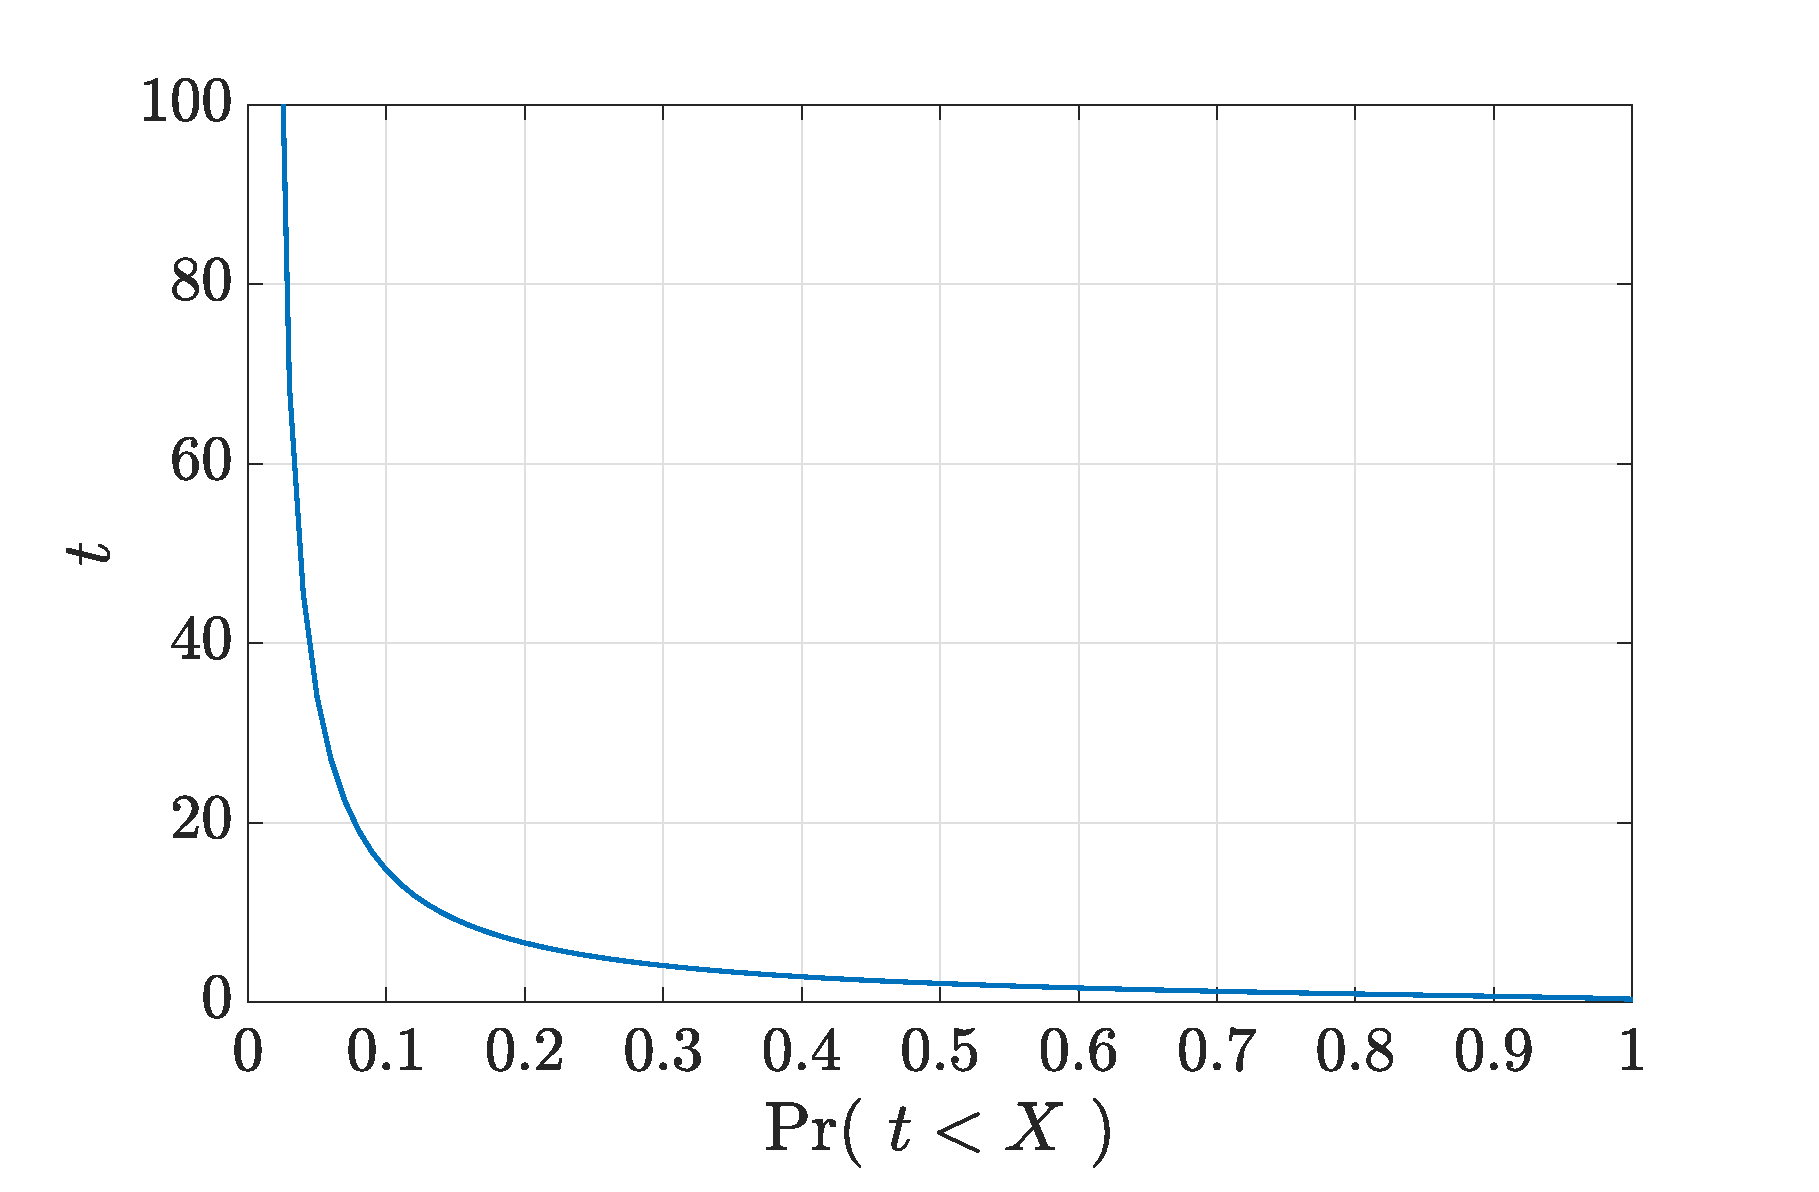
\includegraphics[width = .65\textwidth]{graphs/inverse_chi_square_cdf.eps}}
    \caption{CDF of the inverse chi-square distribution of $\nu = 2$ degrees of freedom.}
    \label{fig:cdf_inverse_chi_square}
\end{figure} 










\subsubsection{LMMSE}
As a recall, the \gls{lmmse} equalizer \textbf{G} needs to satisfy the orthogonality principle. In doing so, we have:
\begin{subequations}
    \begin{align}
         &\EX{(\hat{\textbf{x}}_\text{E} - \textbf{x})\textbf{y}_\text{E}^\text{H}} = \textbf{0} \\
         \Leftrightarrow \; & \EX{(\textbf{G} \textbf{Y}_\text{E}-\textbf{x}) \textbf{y}_\text{E}^\text{H}} = \textbf{0} \\
         \Leftrightarrow \; & \EX{\textbf{G} \textbf{Y}_\text{E} \textbf{y}_\text{E}^\text{H} }  = \EX{\textbf{x} \textbf{y}_\text{E}^\text{H}} \\
         \Leftrightarrow \; & \textbf{G}  = \EX{\textbf{x} \textbf{y}_\text{E}^\text{H}} \left(\EX{\textbf{Y}_\text{E} \textbf{y}_\text{E}^\text{H}}\right)^{-1} \\
         \begin{split}
             \Leftrightarrow \; & \textbf{G}  = \EX{\textbf{x}  \left(   \sqrt{\alpha} \Gamma_{\text{E}} \textbf{x} + \sqrt{1-\alpha} \HE \w + \ve \right)^H }  \\
             & \hspace{.35in} \left(\EX{\left(   \sqrt{\alpha} \Gamma_{\text{E}} \textbf{x} + \sqrt{1-\alpha} \HE \w + \ve \right)\left(   \sqrt{\alpha} \Gamma_{\text{E}} \textbf{x} + \sqrt{1-\alpha} \HE \w + \ve \right)^H}\right)^{-1}
         \end{split}\\
         \begin{split}
            \Leftrightarrow \; & \textbf{G}  = \left(\sqrt{\alpha} \EX{\textbf{xx}^H \Gamma_{\text{E}}^H} + \sqrt{1-\alpha}  \EX{\textbf{x}\w^H \HE^H}  + \EX{x \ve^H}\right) \\
            &\hspace{.35in} \left( \EX{\alpha \Gamma_\text{E} \Gamma_\text{E}^H \textbf{xx}^H + (1-\alpha) \HE \w\w^H\HE^H + \ve\ve^H}\right)^{-1}
         \end{split} \\
         \Leftrightarrow \; & \textbf{G}  = \sqrt{\alpha} \sigma^2_{\text{X}} \Gamma_{\text{E}}^H \left( \alpha \sigma^2_{\text{X}} \Gamma_{\text{E}}\Gamma_{\text{E}}^H  + (1-\alpha) \module{\HE}^2 \sigma^2_{\text{AN}} + \sigma^2_{\text{VE}} \textbf{I}_N\right)^{-1}
    \end{align}
    \label{eq:appA_lmmse}    
\end{subequations}


\newpage
% ANNEXE B : Optimal amout of AN to inject
%\setcounter{figure}{0}
%\setcounter{table}{0}
%\setcounter{section}{0}
%\setcounter{equation}{0}
%\numberwithin{equation}{section}
\renewcommand{\theparagraph}{B}

\section{Optimal amount of AN to inject derivation}\label{appB:alpha}
As a recall, the \gls{sinr} at Bob and Eve are respectively given by:
\begin{equation}
    \begin{split}
        \EX{\gamma_{B,n}} &= \frac{\alpha \;(U+1)}{U \; \sigma_{\text{V,B}}^2} \\
        \EX{\gamma_{E,n}} &= \frac{\alpha}{U(\sigma^2_{\text{V,E}}+(1-\alpha)\sigma^2_{\text{AN}})} 
    \end{split}
\end{equation}
The \gls{sr} becomes:
\begin{subequations}
\begin{align}
    C_s &= \log_2\left(1+ \frac{\alpha (U+1)}{U  \sigma_{\text{V,B}}^2}\right) - \log_2\left(1 + \frac{\alpha}{U(\sigma^2_{\text{V,E}}+(1-\alpha)\sigma^2_{\text{AN}})} \right)\\
    \Leftrightarrow C_s &= \log_2\left( \frac{\alpha (U+1) + U  \sigma_{\text{V,B}}^2}{U  \sigma_{\text{V,B}}^2} \right) - \log_2\left(  \frac{\alpha + U\sigma^2_{\text{V,E}}+(1-\alpha)U\sigma^2_{\text{AN}}}{U\sigma^2_{\text{V,E}}+(1-\alpha)U\sigma^2_{\text{AN}}}  \right)\\
    \Leftrightarrow C_s &= \log_2\left(  \frac{-\alpha^2(U+1)U\sigma^2_{\text{AN}} + \alpha\left[ U(U+1)(\sigma^2_{\text{V,E}}+\sigma^2_{\text{AN}}) - U^2\sigma^2_{\text{V,B}}\sigma^2_{\text{AN}}\right]  + U(\sigma^2_{\text{V,B}}+\sigma^2_{\text{V,E}}+\sigma^2_{\text{AN}})}{\alpha U \sigma^2_{\text{V,B}}(1-U\sigma^2_{\text{AN}}) + U(\sigma^2_{\text{V,B}}+\sigma^2_{\text{V,E}}+\sigma^2_{\text{AN}}) }   \right)
\end{align}
\end{subequations}
If we introduce $T_1=(U+1)U\sigma^2_{\text{AN}}$, $T_2=U(U+1)(\sigma^2_{\text{V,E}}+\sigma^2_{\text{AN}}) - U^2\sigma^2_{\text{V,B}}\sigma^2_{\text{AN}}$, $T_3=U(\sigma^2_{\text{V,B}}+\sigma^2_{\text{V,E}}+\sigma^2_{\text{AN}})$, and $T_4=U \sigma^2_{\text{V,B}}(1-U\sigma^2_{\text{AN}})$, we come back to (\ref{eq:SR_anal2}).

\newpage
% ANNEXE C : Momentum derivation for complex-valued random normal variable 
%\setcounter{figure}{0}
%\setcounter{table}{0}
%\setcounter{section}{0}
%\setcounter{equation}{0}
%\numberwithin{equation}{section}
\renewcommand{\theparagraph}{C}

\section{Momentum computation of complex-valued random normal variables}
\label{appC}
\subsection{Real-valued random normal variable}
For real-valued random variable, the moment-generating function is an alternative specification of its probability distribution. In particular, it allows to compute the moments of the probability distribution as:
\begin{equation}
m_n = \EX{X^n} = M_X^{(n)}(0) = \left. \frac{d^n M_X}{dt^n}\right|_{t=0}
\end{equation}
For a real normal random variable $\mathcal{N}(\mu,\sigma^2) $, the moment-generating function is given by:
\begin{equation}
M_X = e^{t \mu + \frac{1}{2} \sigma^2 t^2 }
\end{equation}
From that, we have:
\begin{equation}
\begin{split}
&\EX{|X|^2} = \sigma^2 + \mu^2\\
&\EX{|X|^4} = 3(\sigma^2)^2 + 6 \sigma^2 \mu^2 + \mu^4
\end{split}
\label{eq:moments_x}
\end{equation}

\subsection{Complex-valued random normal variable}
A complex normal random variable is defined as $Z = X + iY$ where $X \sim \mathcal{N}(\mu_x,\sigma^2_x)$ and $Y \sim \mathcal{N}(\mu_y,\sigma^2_y)$. We also have:
\begin{equation}
\begin{split}
&|Z|^2 = X^2 + Y^2\\
&|Z|^4 = X^4  + 2 X^2 Y^2 + Y^4
\end{split}
\label{eq:deriv_z}
\end{equation}
Since $X$ and $Y$ are independent and taking into account eq.\ref{eq:moments_x}, the moments of $Z$ are easy to compute:
\begin{equation}
\begin{split}
&\EX{|Z|^2} = \sigma_x^2 + \mu_x^2 + \sigma_y^2 + \mu_y^2\\
&\EX{|Z|^4} = 3(\sigma_x^2)^2 + 6 \sigma_x^2 \mu_x^2 + \mu_x^4 + 2\left[ ( \sigma_x^2 + \mu_x^2 )(\sigma_y^2 + \mu_y^2)\right] + 3(\sigma_y^2)^2 + 6 \sigma_y^2 \mu_y^2 + \mu_y^4
\end{split}
\label{eq:moments_z}
\end{equation}






\end{appendices}